\documentclass[../../main/main.tex]{subfiles}
\graphicspath{{./figures/}}

\dominitoc
\faketableofcontents

% \renewcommand{\mtcSfont}{\small\bfseries}
% \renewcommand{\mtcSSfont}{\footnotesize}
\mtcsettitle{minitoc}{}
\mtcsetrules{*}{off}

\makeatletter
\renewcommand{\@chapapp}{\'Electrocin\'etique -- chapitre}
\renewcommand{\chaplett}{E}
\makeatother

% \toggletrue{student}
% \toggletrue{corrige}
% \renewcommand{\mycol}{black}
% \renewcommand{\mycol}{gray}

\hfuzz=5.002pt

\begin{document}
\setcounter{chapter}{4}

\settype{book}
\settype{prof}
\settype{stud}

\chapter{Oscillateur amorti}

\vspace*{\fill}

\begin{tcn}(appl)<ctc>"somm"'t'{Sommaire}
	\let\item\olditem
	\vspace{-15pt}
	\minitoc
	\vspace{-25pt}
\end{tcn}

\begin{tcn}[sidebyside](appl)<ctb>"how"'t'{Capacités exigibles}
	\begin{itemize}[label=\rcheck]
		\item Analyser, sur des relevés expérimentaux, l'évolution de la forme des
		      régimes transitoires en fonction des paramètres caractéristiques.
		\item Prévoir l'évolution du système à partir de considérations
		      énergétiques.
		\item Écrire sous forme canonique l'équation différentielle afin
		      d'identifier la pulsation propre et le facteur de qualité.
		\item Décrire la nature de la réponse en fonction de la valeur du facteur
		      de qualité.
	\end{itemize}
	\tcblower
	\begin{itemize}[label=\rcheck]
		\item Caractériser l'évolution en utilisant les notions d'amplitude, de
		      phase, de période, de fréquence, de pulsation.
		\item Réaliser un bilan énergétique.
		\item Déterminer la réponse détaillée dans le cas d'un régime libre ou
		      d'un système soumis à un échelon en recherchant les racines du
		      polynôme caractéristique.
		\item Déterminer un ordre de grandeur de la durée du régime transitoire
		      selon la valeur du facteur de qualité.
	\end{itemize}
\end{tcn}

\vspace*{\fill}
\newpage
\vspace*{\fill}

%\vspace{-15pt}
\begin{tcn}[%
		sidebyside, fontupper=\small, fontlower=\small
	](appl)<ctb>"chek"'t'{L'essentiel}
	\begin{tcn}[nsp](defi)<ctc>'t'{Définitions}
		\tcblistof[\paragraph*]{defi}{\hspace*{4.8pt}}
	\end{tcn}
	% \begin{tcn}[nsp](rapp)<ctc>'t'{Rappels}
	% 	\tcblistof[\paragraph*]{rapp}{\hspace*{4.8pt}}
	% \end{tcn}
	\begin{tcn}[nsp](prop)<ctc>'t'{Propriétés}
		\tcblistof[\paragraph*]{prop}{\hspace*{4.8pt}}
		% \tcblistof[\paragraph*]{loi}{\hspace*{4.8pt}}
		% \tcblistof[\paragraph*]{theo}{\hspace*{4.8pt}}
	\end{tcn}
	% \begin{tcn}[nsp](loi)<ctc>'t'{Lois}
	% 	\tcblistof[\paragraph*]{loi}{\hspace*{4.8pt}}
	% \end{tcn}
	% \begin{tcn}[nsp](coro)<ctc>'t'{Corollaires}
	%   \tcblistof[\paragraph*]{coro}{\hspace*{4.8pt}}
	% \end{tcn}
	% \begin{tcn}[nsp](demo)<ctc>'t'{Démonstrations}
	% 	\tcblistof[\paragraph*]{demo}{\hspace*{4.8pt}}
	% 	\tcblistof[\paragraph*]{prev}{\hspace*{4.8pt}}
	% \end{tcn}
	% \begin{tcn}[nsp](inte)<ctc>'t'{Interprétations}
	% 	\tcblistof[\paragraph*]{inte}{\hspace*{4.8pt}}
	% \end{tcn}
	% \begin{tcn}[nsp](impl)<ctc>'t'{Implications}
	% 	\tcblistof[\paragraph*]{impl}{\hspace*{4.8pt}}
	% \end{tcn}
	% \begin{tcn}[nsp](tool)<ctc>'t'{Outils}
	% 	\tcblistof[\paragraph*]{tool}{\hspace*{4.8pt}}
	% \end{tcn}
	% \begin{tcn}[nsp](nota)<ctc>'t'{Notations}
	% 	\tcblistof[\paragraph*]{nota}{\hspace*{4.8pt}}
	% \end{tcn}
	% \begin{tcn}[nsp](appl)<ctc>'t'{Applications}
	% 	\tcblistof[\paragraph*]{appl}{\hspace*{4.8pt}}
	% \end{tcn}
	% \begin{tcn}[nsp](rema)<ctc>'t'{Remarques}
	%   \tcblistof[\paragraph*]{rema}{\hspace*{4.8pt}}
	% \end{tcn}
	% \begin{tcn}[nsp](exem)<ctc>'t'{Exemples}
	%   \tcblistof[\paragraph*]{exem}{\hspace*{4.8pt}}
	% \end{tcn}
	% \begin{tcn}[nsp](ror)<ctc>"hart"'t'{Points importants}
	%   \tcblistof[\paragraph*]{ror}{\hspace*{4.8pt}}
	% \end{tcn}
	% \begin{tcn}[nsp](impo)<ctc>'t'{Erreurs communes}
	%   \tcblistof[\paragraph*]{impo}{\hspace*{4.8pt}}
	% \end{tcn}
	\tcblower
	% \begin{tcn}[nsp](defi)<ctc>'t'{Définitions}
	%   \tcblistof[\paragraph*]{defi}{\hspace*{4.8pt}}
	% \end{tcn}
	% \begin{tcn}[nsp](rapp)<ctc>'t'{Rappels}
	%   \tcblistof[\paragraph*]{rapp}{\hspace*{4.8pt}}
	% \end{tcn}
	% \begin{tcn}[nsp](prop)<ctc>'t'{Propriétés}
	% \tcblistof[\paragraph*]{prop}{\hspace*{4.8pt}}
	% \tcblistof[\paragraph*]{loi}{\hspace*{4.8pt}}
	% \tcblistof[\paragraph*]{theo}{\hspace*{4.8pt}}
	% \end{tcn}
	% \begin{tcn}[nsp](coro)<ctc>'t'{Corollaires}
	%   \tcblistof[\paragraph*]{coro}{\hspace*{4.8pt}}
	% \end{tcn}
	\begin{tcn}[nsp](demo)<ctc>'t'{Démonstrations}
		\tcblistof[\paragraph*]{demo}{\hspace*{4.8pt}}
		% \tcblistof[\paragraph*]{prev}{\hspace*{4.8pt}}
	\end{tcn}
	\begin{tcn}[nsp](inte)<ctc>'t'{Interprétations}
		\tcblistof[\paragraph*]{inte}{\hspace*{4.8pt}}
	\end{tcn}
	% \begin{tcn}[nsp](impl)<ctc>'t'{Implications}
	% 	\tcblistof[\paragraph*]{impl}{\hspace*{4.8pt}}
	% \end{tcn}
	% \begin{tcn}[nsp](tool)<ctc>'t'{Outils}
	%   \tcblistof[\paragraph*]{tool}{\hspace*{4.8pt}}
	% \end{tcn}
	% \begin{tcn}[nsp](nota)<ctc>'t'{Notations}
	% 	\tcblistof[\paragraph*]{nota}{\hspace*{4.8pt}}
	% \end{tcn}
	% \begin{tcn}[nsp](odgr)<ctc>'t'{Ordres de grandeur}
	% 	\tcblistof[\paragraph*]{odgr}{\hspace*{4.8pt}}
	% \end{tcn}
	% \begin{tcn}[nsp](appl)<ctc>'t'{Applications}
	% 	\tcblistof[\paragraph*]{appl}{\hspace*{4.8pt}}
	% \end{tcn}
	% \begin{tcn}[nsp](rema)<ctc>'t'{Remarques}
	%   \tcblistof[\paragraph*]{rema}{\hspace*{4.8pt}}
	% \end{tcn}
	% \begin{tcn}[nsp](exem)<ctc>'t'{Exemples}
	% 	\tcblistof[\paragraph*]{exem}{\hspace*{4.8pt}}
	% \end{tcn}
	\begin{tcn}[nsp](ror)<ctc>"hart"'t'{Points importants}
		\tcblistof[\paragraph*]{ror}{\hspace*{4.8pt}}
	\end{tcn}
	\begin{tcn}[nsp](impo)<ctc>'t'{Erreurs communes}
		\tcblistof[\paragraph*]{impo}{\hspace*{4.8pt}}
	\end{tcn}
\end{tcn}

\vspace*{\fill}

\newpage

\section{Oscillateurs amortis}
\subsection{Introduction amorti}

\subsubsection{Évolutions en régime libre, exemple RLC}

\begin{minipage}{0.60\linewidth}
	En reprenant les résultats du LC libre, nous devrions en réalité observer que
	les oscillations dans le circuit s'atténuent. Soit le circuit RLC
	suivant\ftn{\url{https://tinyurl.com/ypbwcwfs}}, avec $L = \SI{43}{mH}$ et $C
		= \SI{20}{nF}$~:
\end{minipage}
\begin{minipage}{0.40\linewidth}
	\begin{center}
		\switch{
			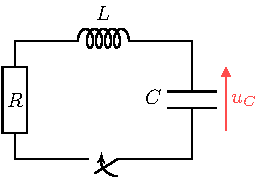
\includegraphics[width=.7\linewidth, draft=true]{rlc_descendant}
		}{
			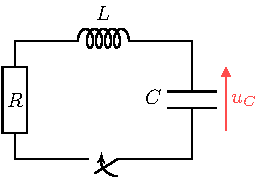
\includegraphics[width=.7\linewidth]{rlc_descendant}
		}
		\captionof{figure}{}
	\end{center}
\end{minipage}

\begin{itemize}
	\item Lorsque la \textbf{résistance est petite}~: on observe \textbf{plusieurs
		      oscillations}.
	      \bigbreak
	      On observe une série d'oscillations à la période $T \approx
		      \SI{184}{\micro s}$. On observe environ 25 oscillations lorsque $R
		      \approx \SI{60}{\ohm}$ (résistance interne du GBF + de la bobine), 9
	      oscillations lorsque $R \approx \SI{180}{\ohm}$, 5 oscillations lorsque
	      $R \approx \SI{500}{\ohm}$.
\end{itemize}
\begin{minipage}{0.45\linewidth}
	\begin{center}
		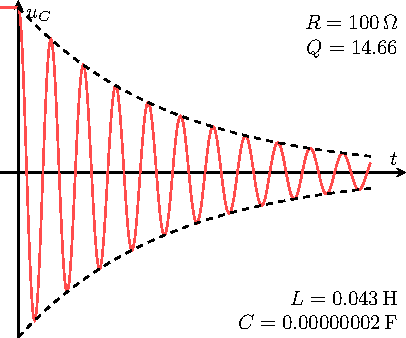
\includegraphics[width=\linewidth]{carac-rlc-15}
	\end{center}
\end{minipage}
\hfill
\begin{minipage}{0.45\linewidth}
	\begin{center}
		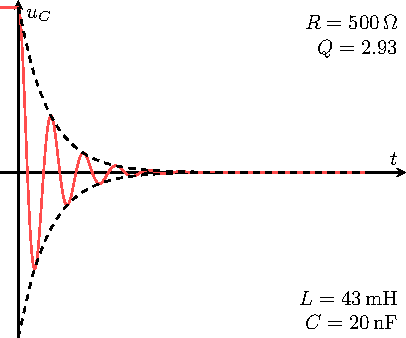
\includegraphics[width=\linewidth]{carac-rlc-3}
	\end{center}
\end{minipage}

\begin{itemize}
	\item Lorsque la \textbf{résistance est plus grande}~: les
	      \textbf{oscillations disparaissent}.
	      \bigbreak
	      Lorsque $R \approx \SI{2,9}{k\ohm}$, on
	      observe un régime transitoire dont la durée est d'environ $\SI{250}{\micro
			      s}$ (à 95\%). Lorsque $R \approx \SI{7.5}{k\ohm}$, on observe un régime
	      transitoire plus long, d'environ \SI{420}{\micro s}.
\end{itemize}
\begin{minipage}{0.45\linewidth}
	\begin{center}
		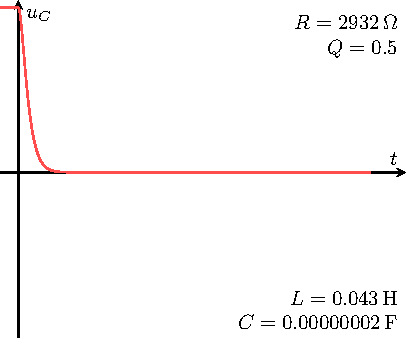
\includegraphics[width=\linewidth]{carac-rlc-05}
	\end{center}
\end{minipage}
\hfill
\begin{minipage}{0.45\linewidth}
	\begin{center}
		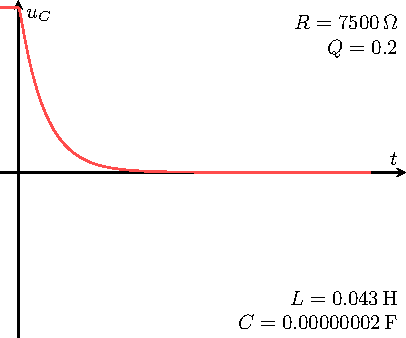
\includegraphics[width=\linewidth]{carac-rlc-02}
	\end{center}
\end{minipage}

\begin{tcb}(expe){Analyse}
	Lorsque l'on excite le système RLC, le système a deux principales réponses~:
	\begin{enumerate}
		\bitem{Système oscillant} pour $R < R_{c}$, de pseudo-période\ftn{On parle
			de \textit{pseudo}-période car le signal est diminué.} \textbf{supérieure à
			$T_0$}~;
		\bitem{Système non-oscillant} pour $R > R_c$~: le transitoire
		\textbf{augmente avec $R$}.
	\end{enumerate}
\end{tcb}

\subsubsection{Équation différentielle}

\begin{tcb}[label=prop:eqdiffoh](prop){Équation différentielle}
	Un oscillateur amorti à un degré de liberté est un système dont l'évolution
	temporelle est décrite par une grandeur $x(t)$ solution d'un équation
	différentielle du type~:
	\psw{
	\[
		\boxed{
		\dv[2]{x}{t} + \frac{\w_0}{Q} \dv{x}{t} + \w_0{}^2x =
		\w_0{}^2x_{\rm eq}
		}
	\]
	}
	Avec $x_{\rm eq}$ la position d'équilibre, $\w_0$ la pulsation
	\textbf{propre}, et $Q >0$ le \textbf{facteur de qualité}, sans dimension.
\end{tcb}
\begin{tcb}[label=impl:eqdiffamorti](impl)<lfnt>{Analyse de l'équation}
	Par lecture de cette équation, avec $Q$ sans dimension on retrouve que
	$\w_0$ s'exprime en \si{s^{-1}} car $\dv{x}{t}$ est de dimension
	$[x]\cdot\si{s^{-1}}$.
	\bigbreak
	De plus, on remarque que \textbf{plus $Q$ est élevé}, plus le terme
	d'ordre 1 est négligeable devant les autres, donc \textbf{plus on se
		rapproche de l'harmonique}.
	\bigbreak
	Le \textbf{facteur de qualité} traduit donc à quel
	point le système est \textbf{idéal}.
\end{tcb}

\subsubsection{Équation caractéristique et régimes de solutions}
\begin{tcb}[label=def:eqcarac, sidebyside](defi){Équation caractéristique}
	Pour résoudre une équation différentielle, on suppose une solution de la
	forme $x(t) = A\exp(rt)$ avec $r \in \Cb$. En injectant cette
	expression dans l'équation différentielle, on obtient l'\textbf{équation
		caractéristique}~:
	\psw{
		\begin{equation*}
			\boxed{r^2 + \frac{\w_0}{Q}r + \w_0{}^2 = 0}
		\end{equation*}
	}
	\tcblower
	C'est un trinôme du second degré, dont le discriminant $\Delta$ est
	\psw{
		\begin{equation*}
			\boxed{
				\Delta =
				\left( \frac{\w_0}{Q} \right)^2 - 4\w_0{}^2 =
				\frac{\w_0{}^{2}}{Q^{2}}\left( 1-4Q^{2} \right)
			}
		\end{equation*}
	}
\end{tcb}
\begin{tcb}[label=impl:eqcarac](impl){Régimes de solutions}
	Selon la valeur du discriminant, on aura différentes valeurs de $r$,
	doubles réelles, simple réelle ou doubles complexes. On a en effet
	\psw{
		\begin{gather*}
			\Delta > 0
			\Lra
			\cancel{\frac{w_0{}^{2}}{Q^{2}}}\left( 1-4Q^{2} \right) >0
			\Lra
			4Q^2 < 1
			\Lra
			Q < \frac{1}{2}
		\end{gather*}
	}
	\vspace{-15pt}
	\begin{description}
		\item[$\mathbf{Q > 1/2}$] : régime \textbf{pseudo-périodique},
		      racines complexes et oscillations décroissantes~;
		\item[$\mathbf{Q = 1/2}$] : régime \textbf{critique}, racine double
		      réelle~;
		\item[$\mathbf{Q < 1/2}$] : régime \textbf{apériodique}, racines
		      réelles et décroissance exponentielle sans oscillation.
	\end{description}
\end{tcb}

\begin{tcb}[label=nota:pm](nota){$\pm$ et $\mp$}
	Il est courant de noter les racines $r_\pm$ pour dénoter à la fois $r_+$ et
	$r_-$. Dans ce cas, l'expression de la racine contient le signe $\pm$, ce
	qui signifie que $r_+$ correspond à l'expression avec le $+$, et $r_-$
	correspond à l'expression avec le $-$.
	\smallbreak
	Si l'expression contient le signe $\mp$, c'est l'opposé~: $r_+$ correspond à
	l'expression avec $-$.
\end{tcb}

\begin{tcb}[label=prop:solureg, tabularx={Y|Y|Y}](ror){Solutions}
	\textbf{Pseudo-périodique} & \textbf{Critique} & \textbf{Apériodique}
	\\\hline
	$\D < 0 \Lra Q > 1/2$ & $\D = 0 \Lra Q = 1/2$ & $\D >
		0 \Lra Q < 1/2$
	\\\hline
	\begin{equation*}
		\boxed{r_\pm = - \frac{\w_0}{2Q} \pm \jj\W}
	\end{equation*}
	\begin{equation*}
		\boxed{\W = \frac{\w_0}{2Q}\sqrt{4Q^2 - 1}}
	\end{equation*}
	&
	\begin{equation*}
		\boxed{r = - \frac{\w_0}{2Q} = -\w_0}
	\end{equation*}
	&
	\begin{equation*}
		\boxed{r_\pm = \frac{\w_0}{2Q}\left(-1 \pm \sqrt{1 - 4Q^2}\right)}
	\end{equation*}
	\\\hline
	\begin{empheq}[box=\fbox]{gather*}
		x(t) = \underbrace{\exp \left(-\frac{\w_0}{2Q}t\right)}_{
			\text{partie décroissante}}\times\\
		\underbrace{\left[ A\cos(\Wt) + B\sin(\Wt) \right]}_{
			\text{partie oscillante}}
	\end{empheq}
	&
	\begin{equation*}
		\boxed{x(t) = (At + B)\exp(-\w_0t)}
	\end{equation*}
	&
	\begin{empheq}[box=\fbox]{gather*}
		x(t) = A\exp(r_+t) +\\
		\hspace{26pt} B\exp(r_-t)
	\end{empheq}
	\\
\end{tcb}

\subsection{Oscillateur amorti électrique~: circuit RLC série libre}
\subsubsection{Présentation}
\begin{minipage}[c]{.6\linewidth}
	\begin{itemize}
		\item Il est constitué de l'association en série d'une résistance, d'une
		      bobine et d'un condensateur idéaux.
		\item \textbf{On suppose le condensateur initialement chargé}~:
		      \fbox{$u_C(0^-) = E$ \underline{et} $i(0^-) = 0$} (condensateur chargé
		      $\equiv$ interrupteur ouvert).
		\item À $t=0$, on coupe le générateur.
	\end{itemize}
\end{minipage}
\hfill
\begin{minipage}[c]{.35\linewidth}
	~
	\begin{center}
		\switch{
			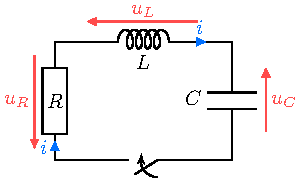
\includegraphics[width=.9\linewidth, draft=true]{rlc_descendant-intens}
		}{
			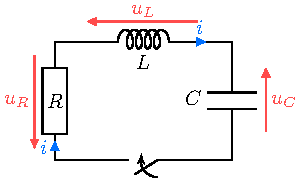
\includegraphics[width=.9\linewidth]{rlc_descendant-intens}
		}
		\captionof{figure}{}
	\end{center}
\end{minipage}

\subsubsection{Bilan énergétique}
\begin{tcb}[label=demo:rcenerg-charge](demo)<lfnt>{Bilan d'énergie}
	On fait un bilan de puissances~:
	\psw{
		\begin{DispWithArrows*}
			u_Ci + u_Li + u_Ri &= 0
			\Arrow{$i = C \dv{u_C}{t}$, $u_L = L \dv{i}{t}$ et $u_R = Ri$}
			\\\Lra
			u_C\times C \dv{u_C}{t} + L \dv{i}{t}\times i + Ri^2 &= 0
			\Arrow{$\Pc_J = Ri^{2}$ et $f \times f' = \left(\frac{1}{2}f^{2}\right)'$}
			\\\Lra
			\dv{}{t}
			\Big(
			\underbracket[1pt]{\frac{1}{2}C  u_C{}^2}_{\Ec_C} +
			\underbracket[1pt]{\frac{1}{2}Li^2}_{\Ec_L}
			\Big) &= -\Pc_J
		\end{DispWithArrows*}
	}
	\vspace{-15pt}
\end{tcb}
\begin{tcb}[label=prop:lcenerg-décharge](prop){Bilan d'énergie}
	L'énergie emmagasinée dans le circuit est progressivement dissipée par
	effet \textsc{Joule} dû à la résistance~:
	\psw{
		\[
			\boxed{\dv{\Ec}{t} = -\Pc_J}
		\]
	}
	avec $\Ec = \Ec_C + \Ec_L = \frac{1}{2}Cu_C{}^2 + \frac{1}{2}Li^2$.
\end{tcb}
\begin{tcb}[label=impo:amortissement, cnt, bld](impo){Résultat}
	On a donc bien une perte d'énergie à cause de la dissipation dans la
	résistance. Il y aura donc progressivement une perte de la tension
	de $u_C$, d'où l'amortissement.
\end{tcb}

\subsubsection{Équation différentielle du circuit}
\begin{tcb}[label=demo:eqdiffrc, sidebyside](demo)<lfnt>{Équation diff. RLC libre}
	Avec la loi des mailles,
	\psw{
		\begin{DispWithArrows*}[fleqn, mathindent=2pt]
			u_L + u_R + u_C &= 0
			\Arrow{$u_L = L \dv{i}{t}$\\et $u_R = Ri$}
			\\\Lra
			L \dv{i}{t} + Ri + u_C &= 0
			\Arrow{$i = C \dv{u_C}{t}$}
			\\\Lra
			LC \dv[2]{u_C}{t} + RC \dv{u_C}{t} + u_C                   &= 0
			\Arrow{forme\\canonique}
			\\
			\Lra \dv[2]{u_C}{t} + \frac{R}{L} \dv{u_C}{t} + \frac{1}{LC}u_C &= 0
		\end{DispWithArrows*}
	}
	\tcblower
	On détermine l'expression de $Q$ par identification~:
	\psw{
		\begin{DispWithArrows*}
			\frac{\w_0}{Q} &= \frac{R}{L}
			\Arrow{$\w_0 = \frac{1}{\sqrt{LC}}$}
			\\\Lra
			\frac{1}{Q \sqrt{LC}} &= \frac{R}{L}
			\Arrow{On isole $Q$}
			\\\Lra
			Q &= \frac{L}{R \sqrt{LC}}
			\Arrow{$L = \sqrt{L}^{2}$}
			\\\Lra
			\Aboxed{Q &= \frac{1}{R}\sqrt{\frac{L}{C}}}
		\end{DispWithArrows*}
	}
\end{tcb}
\begin{tcb}[label=prop:eqdiffrc, sidebyside,
		righthand ratio=.4](prop){Équation diff. RLC libre}
	L'équation différentielle de la tension $u_C(t)$ aux bornes d'un
	condensateur dans un circuit RLC en régime libre est
	\psw{
		\[
			\boxed{\dv[2]{u_C}{t} + \frac{\w_0}{Q} \dv{u_C}{t} + \w_0{}^2u_C = 0}
		\]
	}
	\begin{itemize}
		\item \fbox{$\w_0 = \frac{1}{\sqrt{LC}}$} la pulsation propre~;
		\item \fbox{$Q = \frac{1}{R} \sqrt{\frac{L}{C}}$} le facteur de
		      qualité.
	\end{itemize}
	\tcblower
	Les conditions initiales (continuité de $u_C$ aux bornes de $C$
	et de $i$ traversant $L$) sont
	\psw{
		\begin{empheq}[box=\fbox]{gather*}
			u_C(0^-) = u_C(0^+) = E\\
			i(0^-) = i(0^+) = 0
		\end{empheq}
	}
\end{tcb}

\subsubsection{Solutions}
\paragraph{Cas $\D < 0 \Lra Q > 1/2$~: régime pseudo-périodique}
~ \smallbreak
\begin{tcb}[label=demo:solupseudoper, breakable](demo)<lfnt>{Solution}
	On part de l'équation caractéristique~:
	\psw{
		\[
			r^{2} + \frac{\w_0}{Q}r + \w_0{}^{2} = 0
		\]
	}
	\vspace{-15pt}
	On a donc, avec $Q > 1/2$,
	\psw{
		\[
			\Delta = \frac{\w_0{}^{2}}{Q^{2}}\left( 1-4Q^{2} \right) < 0
		\]
	}
	\vspace{-15pt}
	Ainsi,
	\psw{
		\begin{DispWithArrows*}
			r_\pm & = \frac{-\frac{\w_0}{Q} \pm \jj\sqrt{-\D}}{2}
			\Arrow{On injecte $\Delta$}
			\\\Lra
			r_\pm &= -\frac{\w_0}{2Q} \pm
			\frac{\jj}{2} \sqrt{\frac{\w_0{}^{2}}{Q^{2}}\left( 4Q^{2}-1 \right)}
			\Arrow{On extrait $\frac{\w_0}{Q}$}
			\\\Lra
			r_\pm &= - \frac{\w_0}{2Q} \pm \jj \frac{\w_0}{2Q} \sqrt{4Q^{2}-1}
			\Arrow{On définit $\W$}
			\\\Lra
			r_\pm &= - \frac{\w_0}{2Q} \pm \jj\W
		\end{DispWithArrows*}
	}
	d'où la définition de $\W$~:
	\[
		\boxed{\W = \frac{\w_0}{2Q}\sqrt{4Q^{2}-1}}
	\]
	Ensuite, avec la forme générale de la solution on a
	\psw{
		\begin{equation*}
			u_C(t) = \exp \left(-\frac{\w_0}{2Q}t\right)
			\left[ A\cos(\Wt) + B\sin(\Wt) \right]
		\end{equation*}
	}
	\vspace{-15pt}
	\begin{itemize}
		\item On trouve $A$ avec la première condition initiale~:
		      \psw{
			      \begin{gather*}
				      u_C(0) = E = 1 \left[ A \cdot 1 + B \cdot 0 \right] = A
				      \quad \Ra \quad \boxed{A=E}
			      \end{gather*}
		      }
		      \vspace{-15pt}
		\item On trouve $B$ avec la seconde CI~:
		      \psw{
			      \begin{gather*}
				      \hspace*{-10pt}
				      \dv{u_C}{t} =
				      -\frac{\w_0}{2Q}\exp \left( -\frac{\w_0}{2Q}t \right)\times
				      \left[ A\cos(\Wt) + B\sin(\Wt) \right] +
				      \exp \left( -\frac{\w_0}{2Q}t \right)
				      \left[ -A\W\sin(\Wt) + B\W\cos(\Wt) \right]
				      \\\Ra
				      \dv{u_C}{t}\/(0) = - \frac{\w_0}{2Q}A + \W B = 0
				      \\\Lra
				      \boxed{B = \frac{\w_0}{2Q\W}E = \frac{E}{\sqrt{4Q^2-1}}}
			      \end{gather*}
		      }
	\end{itemize}
	% Ainsi, on trouve bien
	% \begin{empheq}[box=\fbox]{gather*}
	% 	u_C(t) = E\exp \left( -\frac{\w_0}{2Q}t \right)\times
	% 	\left[
	% 		\cos(\Wt) + \frac{1}{\sqrt{4Q^2 - 1}}\sin(\Wt)
	% 		\right]
	% \end{empheq}
\end{tcb}
\begin{tcb}[label=prop:solupseudoper, sidebyside](prop){Solution}
	Pour un facteur de qualité $Q > 1/2$, $u_C$ s'exprime par
	\psw{
		\begin{empheq}[box=\fbox]{gather*}
			u_C(t) = E\exp \left( -\frac{\w_0}{2Q}t \right)\times\\
			\left[
				\cos(\Wt) + \frac{1}{\sqrt{4Q^2 - 1}}\sin(\Wt)
				\right]
		\end{empheq}
	}
	avec
	\begin{equation*}
		\boxed{\W = \frac{\w_0}{2Q} \sqrt{4Q^2 - 1}}
	\end{equation*}
	La période des oscillations \textbf{diffère des oscillations harmoniques} $T_0
		= 2\pi/\w_0$ selon
	\psw{
		\begin{equation*}
			\boxed{
				T =
				\frac{2\pi}{\W} =
				\frac{2\pi}{\w_0} \frac{2Q}{\sqrt{4Q^{2} - 1}}
			}
		\end{equation*}
	}
	\tcblower
	Les oscillations se font entre les courbes
	\[y(t) = \pm E \exp \left( - \frac{\w_0}{2Q}t \right)\]
	\begin{center}
		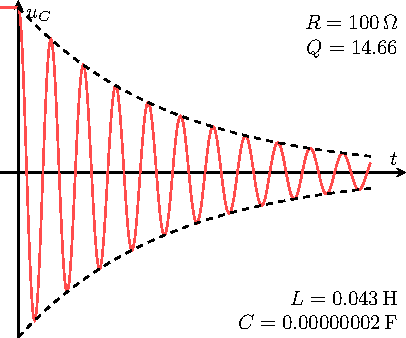
\includegraphics[width=\linewidth]{carac-rlc-15}
		\captionof{figure}{}
	\end{center}
\end{tcb}

\begin{tcb}[label=demo:transipseudo](demo)<lfnt>{Régime transitoire}
	L'amplitude varie selon $E\exp \DS \left( -\frac{\w_0}{2Q}t \right)$~; on
	définit donc $t_{95}$ tel que
	\psw{
		\begin{DispWithArrows*}
			\exp \left(-\frac{\w_0}{2Q}t_{95} \right) &= 0.05
			\Arrow{$\ln (~)$}
			\\\Lra
			- \frac{\w_0}{2Q}t_{95} &= \ln(0.05)
			\Arrow{$0.05 = 1/20$ et $\ln (a^{b}) = b \ln a$}
			\\\Lra
			\frac{\w_0}{2Q}t_{95} &= \ln(20)
			\Arrow{On isole}
			\\\Lra
			t_{95} &= 2\ln(20) \frac{Q}{\w_0}
		\end{DispWithArrows*}
	}
	Or $2\ln(20) \approx 2\pi$, d'où
\end{tcb}
\begin{tcb}[label=prop:transipseudo](prop)<lfnt>{Régime transitoire}
	Le temps de réponse à 95\% est atteint à partir de $t_{95}$ tel que
	\psw{
		\begin{equation*}
			\boxed{t_{95} \approx QT_0} \qav \boxed{T_0 = \frac{2\pi}{\w_0}}
		\end{equation*}
	}
	\vspace{-15pt}
\end{tcb}
\begin{tcb}[label=impo:pseudograndQ](impo){Résultat à grand $Q$}
	Avec ces résultats on remarque en effet que quand $Q \rightarrow \infty$, on
	a à la fois
	\begin{equation*}
		\boxed{\W \approx \w_0} \qdc \boxed{T \approx T_0}
	\end{equation*}
	Mais aussi
	\begin{equation*}
		\boxed{\dv[2]{u_C}{t} + \w_0{}^2u_C = 0} \qdc \boxed{u_C(t) = E\cos(\w_0t)}
	\end{equation*}
	On retrouve toutes les caractéristiques de la situation harmonique.
\end{tcb}

\begin{tcb}[breakable](rema){Visualisation dans l'espace des phases}
	Contrairement à la situation harmonique, le tracé de la solution dans
	l'espace $(u_C,i)$ n'est \textbf{pas symétrique par inversion du temps}~: la
	dissipation par effet \textsc{Joule} diminue l'énergie du système, et la
	\textbf{tension diminue progressivement}.
	\bigbreak
	On observera donc une \textbf{spirale décroissante} avec beaucoup
	d'oscillations quand les amortissements ne sont pas trop élevés, et de moins
	en moins quand $Q$ diminue ou que l'amortissement augmente.
	\tcblower
	\noindent
	\begin{minipage}{0.49\linewidth}
		\begin{center}
			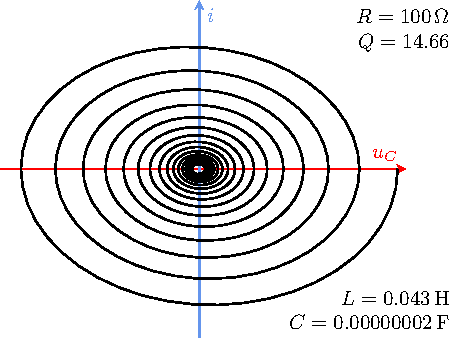
\includegraphics[width=.7\linewidth]{carac-rlc_xy-15}
			\captionof{figure}{Faible amortissement}
		\end{center}
	\end{minipage}
	\begin{minipage}{0.49\linewidth}
		\begin{center}
			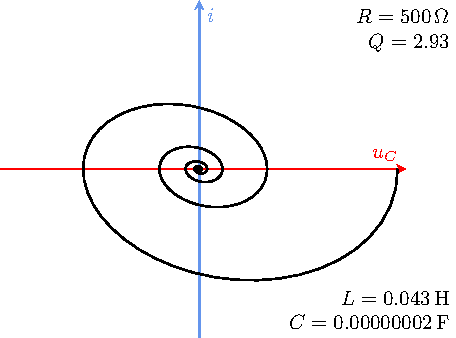
\includegraphics[width=.7\linewidth]{carac-rlc_xy-3}
			\captionof{figure}{Moyen amortissement}
		\end{center}
	\end{minipage}
\end{tcb}

\newpage
\paragraph{Cas $\D = 0 \Lra Q = 1/2$~: régime critique}
~\smallbreak
\vspace{-15pt}
\begin{tcb}[label=demo:solupseudoper](demo)<lfnt>{Solution}
	La seule racine de l'équation caractéristique est double, et vaut
	\psw{
		\[
			r = -\w_0
		\]
	}
	Ensuite, avec la forme générale de la solution on a
	\psw{
		\begin{equation*}
			u_C(t) = (At+B)\exp \left(-\w_0t\right)
		\end{equation*}
	}
	\vspace{-20pt}
	\begin{itemize}
		\item On trouve $B$ avec la première condition initiale~:
		      \psw{
			      \begin{gather*}
				      u_C(0) = E = (A\cdot0 + B)\cdot1 = B
				      \quad \Ra \quad \boxed{B=E}
			      \end{gather*}
		      }
		      \vspace{-15pt}
		\item On trouve $A$ avec la seconde CI~:
		      \psw{
			      \begin{gather*}
				      \dv{u_C}{t} = (A)\exp(-\w_0t) +
				      (At+E)(-\w_0)\exp(-\w_0t)
				      \\\Ra
				      \dv{u_C}{t}\/(0) = A -\w_0E = 0
				      \\\Lra
				      \boxed{A = \w_0E}
			      \end{gather*}
		      }
		      \vspace{-15pt}
	\end{itemize}
	\vspace{-30pt}
\end{tcb}
\begin{tcb}[label=prop:solupseudoper, sidebyside](prop){Solution}
	Pour un facteur de qualité $Q = 1/2$, $u_C$ s'exprime par
	\psw{
		\begin{empheq}[box=\fbox]{gather*}
			u_C(t) = E(\w_0t + 1) \exp(-\w_0t)
		\end{empheq}
	}
	et on n'observe \textbf{pas une oscillation}.
	\tcblower
	\begin{center}
		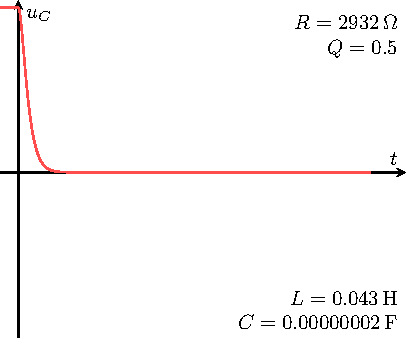
\includegraphics[width=\linewidth]{carac-rlc-05}
		\captionof{figure}{}
	\end{center}
\end{tcb}
\begin{tcb}[sidebyside](exem){Visualisation dans l'espace des phases}
	Au facteur de qualité critique, l'amortissement est suffisamment important
	pour empêcher $u_C$ de passer sous 0.
	\tcblower
	\begin{center}
		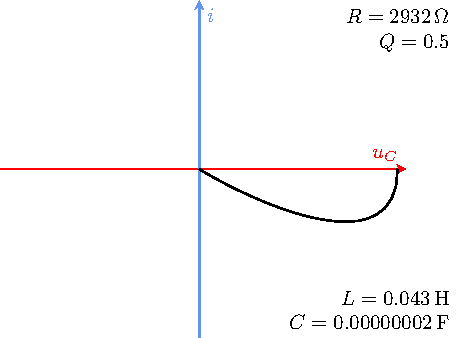
\includegraphics[width=.9\linewidth]{carac-rlc_xy-05}
		\captionof{figure}{}
	\end{center}
\end{tcb}
\begin{tcb}[label=demo:transicrit](demo)<lfnt>{Régime transitoire}
	En négligeant le terme linéaire en $t$ devant la décroissance
	exponentielle, on a
	\psw{
		\begin{gather*}
			\exp (-\w_0t_{95}) = \num{0.05} \Lra t_{95} =
			\frac{\ln(20)}{\w_0}
		\end{gather*}
	}
	\vspace{-15pt}
	Et avec $\ln(20) \approx \pi$ on a~:
\end{tcb}
\begin{tcb}[label=prop:transicrit](prop)<lfnt>{Régime transitoire}
	Le temps de réponse à 95\% est atteint à partir de $t_{95}$ tel que
	\psw{
		\begin{equation*}
			\boxed{t_{95} \approx \frac{T_0}{2}} \qav \boxed{T_0 = \frac{2\pi}{\w_0}}
		\end{equation*}
	}
	\vspace{-15pt}
\end{tcb}

\paragraph{Cas $\D > 0$~: régime apériodique}
~\smallbreak
\begin{tcb}[label=demo:solupseudoper, sidebyside](demo)<lfnt>{Solution}
	Les racines de l'équation caractéristique sont réelles, et on a
	\psw{
		\begin{gather*}
			r_\pm =
			\frac{- \frac{\w_0}{2Q}\pm\sqrt{\Delta}}{2}
			\\\Lra
			r_\pm = - \frac{\w_0}{2Q} \pm \frac{\w_0}{2Q} \sqrt{1 - 4Q^2}
			\\\Lra
			r_\pm = \frac{\w_0}{2Q} \left(-1 \pm \sqrt{1 - 4Q^2} \right)
		\end{gather*}
	}
	Ensuite, avec la forme générale de la solution on a
	\psw{
		\begin{equation*}
			u_C(t) = A \exp(r_+t) + B\exp(r_-t)
		\end{equation*}
	}
	\vspace{-15pt}
	\tcblower
	\begin{itemize}
		\item Avec la première CI~:
		      \psw{
			      \begin{gather*}
				      u_C(0) = E = A + B
			      \end{gather*}
		      }
		      \vspace{-15pt}
		\item Avec la seconde CI~:
		      \psw{
			      \begin{gather*}
				      \dv{u_C}{t}\/(0) = Ar_+ + Br_- = 0
				      \\\Lra
				      B = - \frac{Ar_+}{r_-}
			      \end{gather*}
		      }
		      \vspace{-15pt}
	\end{itemize}
	En combinant, on trouve
	\begin{equation*}
		\psw{
			\boxed{A = - \frac{Er_-}{r_+ - r_-}}
		}
		\qet
		\psw{
			\boxed{B = \frac{Er_+}{r_+ - r_-}
			}
		}
	\end{equation*}
	D'où le résultat~:
\end{tcb}
\begin{tcb}[label=prop:solupseudoper, sidebyside](prop){Solution}
	Pour un facteur de qualité $Q < 1/2$, $u_C$ s'exprime par
	\psw{
		\[
			\boxed{
				u_C(t) =
				\frac{E}{r_+-r_-} \left( r_+\exp(r_-t) - r_-\exp(r_+t) \right)
			}
		\]
	}
	et on n'observe \textbf{pas une oscillation}. Le régime transitoire est
	\textit{plus long} que pour $Q = 1/2$.
	\tcblower
	\begin{center}
		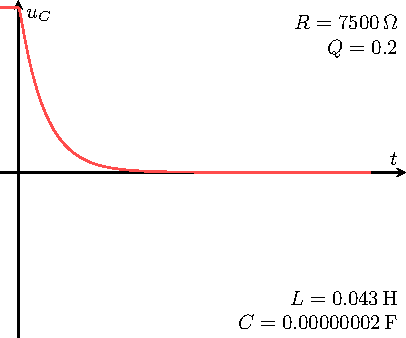
\includegraphics[width=\linewidth]{carac-rlc-02}
		\captionof{figure}{}
	\end{center}
\end{tcb}

\begin{tcb}[sidebyside](exem){Visualisation dans l'espace des phases}
	Pendant le régime apériodique, l'amortissement est suffisamment important pour
	non seulement empêcher $u_C$ d'osciller, mais également pour \textbf{ralentir
		sa diminution }vers $0$. Son trajet se fait donc à une vitesse plus faible,
	c'est-à-dire $\dv{u_C}{t}$ plus petit donc $i$ plus petit.
	\tcblower
	\begin{center}
		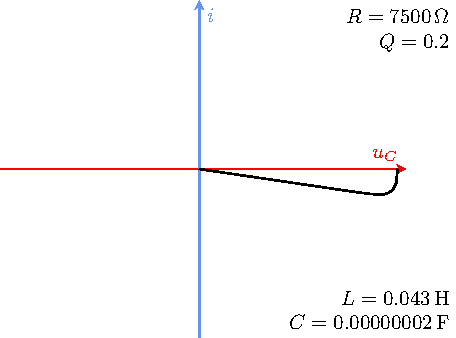
\includegraphics[width=\linewidth]{carac-rlc_xy-02}
		\captionof{figure}{}
	\end{center}
\end{tcb}
\begin{tcb}[label=demo:transiaper](demo)<lfnt>{Régime transitoire}
	La décroissance sera guidée par l'exponentielle la «~\textbf{moins
		décroissante}~». On cherche donc à savoir laquelle, on compare donc $r_-$ et
	$r_+$.
	\smallbreak
	On remarque d'abord que les deux racines sont négatives (d'où la
	décroissance exponentielle). En effet,
	\vspace{-15pt}
	\psw{
		\begin{align*}
			r_+ < 0
			 & \Lra
			\underbrace{\cancel{-\frac{\w_0}{2Q}}}_{\w_0 \text{ et } Q > 0}
			\left( 1 - \sqrt{1-4Q^2}
			\right) \underbrace{\cancel{<}}_{>} 0
			\\&\Lra
			1 - \sqrt{1 - 4Q^2} > 0
			\\&\Lra
			\sqrt{1-4Q^2}^{2} < 1^{2}
			\\&\Lra
			4Q^2 > 0
		\end{align*}
	}
	\vspace{-15pt}
	ce qui est vrai. Or,
	\psw{
		\begin{DispWithArrows*}[]
			r_- &< r_+
			\Arrow{$\abs{~}$}
			\\\Lra
			\abs{r_-} &> \abs{r_+}
			\Arrow{$(~)^{-1}$}
			\\\Lra
			\abs{\frac{1}{r_-}} &< \abs{\frac{1}{r_+}}
			\Arrow{$\tau = \abs{1/r}$}
			\\\Lra
			\tau_- &< \tau_+
		\end{DispWithArrows*}
	}
	On estime alors la durée du régime transitoire à
	\fbox{$\ln(20)/\abs{r_+}$}.
	\bigbreak
	Pour $Q \ll 1$, on utilise \fbox{$\sqrt{1+x} \underset{x\ll1}{\approx}
			1+x/2$} pour simplifier $r_+$~:
	\psw{
		\begin{gather*}
			r_+ =
			-\frac{\w_0}{2Q} \left( 1 - \sqrt{1-4Q^{2}} \right)
			\\\Ra
			r_+ \underset{Q\ll1}{\approx}
			- \frac{\w_0}{2Q} \left( 1 - \left(1 - \frac{4Q^2}{2}\right) \right)
			\\\Lra
			r_+ \underset{Q\ll1}{\approx} -Q\w_0
		\end{gather*}
	}
	Avec $\ln(20) \approx \pi$, on a finalement
	\psw{
		\begin{equation*}
			\boxed{t_{95} \approx \frac{\pi}{Q\w_0}} \qso \boxed{t_{95} \approx
				\frac{T_0}{2Q}}
		\end{equation*}
	}
	\vspace{-15pt}
\end{tcb}

\begin{tcb}[label=prop:transiaper](prop)<lfnt>{Régime transitoire}
	Le temps de réponse à 95\% est atteint à partir de $t_{95}$ tel que
	\psw{
		\begin{equation*}
			\boxed{
				t_{95} \approx \frac{T_0}{2Q}} \qav \boxed{T_0 =
				\frac{2\pi}{\w_0}
			}
		\end{equation*}
	}
\end{tcb}
\begin{tcb}[label=impo:aperpetitQ](impo){Résultat à faible $Q$}
	Quand $Q \longrightarrow 0$, on peut négliger le terme d'ordre 2 dans
	l'équation différentielle, soit
	\begin{gather*}
		\frac{\cancel{\w_0}}{Q}\dv{u_C}{t} +
		\w_0{}^{\cancel{2}}u_C = R \sqrt{\frac{C}{L}} \dv{u_C}{t} +
		\frac{1}{\sqrt{LC}}u_C \\
		=
		\dv{u_C}{t} + \frac{1}{R}
		\sqrt{\frac{\bcancel{L}}{\bcancel{L}C^2}} u_C
		=
		\boxed{ \dv{u_C}{t} +
			\frac{1}{RC} u_C}
	\end{gather*}
	d'où la décroissance exponentielle. D'autre part, les valeurs de $r_\pm$
	tendent vers la même valeur $r = - \frac{\w_0}{2Q}$~: en supposant la solution
	comme la somme des deux racines, on aurait une décroissance en
	\begin{gather*}
		r = -\frac{\w_0}{Q} = - \frac{1}{\sqrt{LC}}R
		\sqrt{\frac{C}{L}}
		\Lra
		r = -R \sqrt{\frac{\cancel{C}}{L^2\cancel{C}}}
	\end{gather*}
	soit une décroissance exponentielle avec un temps
	caractéristique $\tau = \frac{L}{R}$.
\end{tcb}

\vspace{-15pt}
\subsection{Exemple amorti mécanique~: ressort + frottements fluides}

\subsubsection{Présentation}
\begin{tcb}[label=def:ressortlibre, sidebyside](defi){Situation
			initiale et bilan des forces}
	\begin{itemize}[label=$\diamond$, leftmargin=10pt]
		\bitem{Système~:} \{point M\} de masse $m$, accroché à un \textbf{ressort
			idéal avec frottements}
		\bitem{Référentiel~:} $\Rc\ind{sol}(O',x,y,t)$ supposé galiléen
		\bitem{Repère~:} $(\Or', \ux, \uy)$ (voir schéma)
		\bitem{Repérage~:}
		\vspace{-15pt}
		\begin{center}
			\hspace*{-10pt}
			\fbox{Soit $x (t) = \ell(t) - \ell_0$ la position de la masse}
		\end{center}
		\[
			\vv{\rm O'M} = x(t)\ux~; \vf = \xp(t)\ux~; \af = \xpp(t)\ux.
		\]
		\bitem{Position initiale~:} ${\rm O'M}(0) = x_0 >0$
		\bitem{Vitesse initiale~:} $\vf(0) = \of$
	\end{itemize}
	\tcblower
	\begin{center}
		\switch{
			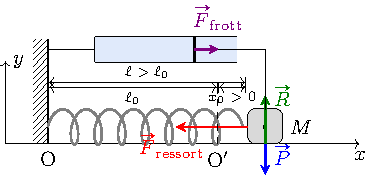
\includegraphics[width=\linewidth, draft=true]{ressort_amorti}
		}{
			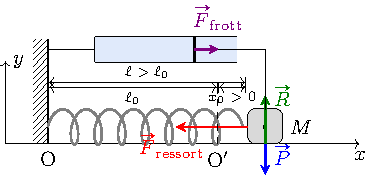
\includegraphics[width=\linewidth]{ressort_amorti}
		}
		\captionof{figure}{}
	\end{center}
	\begin{itemize}[label=$\diamond$, leftmargin=10pt]
		\bitem{Bilan des forces~:}
		\psw{
			\[
				\begin{array}{ll}
					\textbf{Poids}               & \Pf = m\gf = -mg \uy         \\
					\textbf{Réaction normale}    & \Rf = R\uy                   \\
					\textbf{Force de rappel}     & \Ff = -kx (t)\ux             \\
					\textbf{Force de frottement} & \Ff_{\rm frott} = -\alpha\vf
				\end{array}
			\]
		}
	\end{itemize}
\end{tcb}

\subsubsection{Équation différentielle}

\begin{tcbraster}[raster columns=2, raster equal height=rows]
	\begin{tcb}[label=prop:eqdiffreslibre](prop){Équation et solution}
		La position $x$ de la masse et la longueur $\ell$ du ressort sont régies
		par~:

		\begin{empheq}[box=\fbox]{gather*}
			\dv[2]{x}{t} + \frac{\w_0}{Q} \dv{x}{t} + \w_0{}^2x = 0\\
			\Lra \dv[2]{\ell}{t} +
			\frac{\w_0}{Q} \dv{\ell}{t} + \w_0{}^2\ell = \w_0{}^2\ell_0
		\end{empheq}
		\begin{itemize}
			\item \fbox{$\w_0 = \frac{k}{m}$} la pulsation propre~;
			\item \fbox{$Q = \frac{\sqrt{km}}{\alpha}$} le facteur de qualité.
		\end{itemize}
		$\ell_0$ \textbf{reste} donc la longueur d'équilibre du système.
	\end{tcb}
	\begin{tcb}[label=demo:solreslibre](demo)'r'{Équation différentielle}
		Avec le PFD~:
		\psw{
			\begin{gather*}
				m\af = \Pf + \vv{R} + \Ff\\
				\Lra m\left(
				\begin{array}{c}
						\dv[2]{x}{t} \\
						0
					\end{array}
				\right)
				=
				\left(
				\begin{array}{c}
						-kx -\alpha v \\
						-mg + R
					\end{array}
				\right)
			\end{gather*}
		}
		Sur l'axe $\ux$ on trouve donc
		\psw{
			\[
				m \dv[2]{x}{t} + \alpha \dv{x}{t} + kx = 0
			\]
		}
		\vspace{-15pt}
	\end{tcb}
\end{tcbraster}

\begin{tcb}[sidebyside, righthand ratio=.4](impo){Analogie RLC-ressort amorti}
	Ici aussi, les deux systèmes sont \textbf{régis par la même équation
		différentielle}. On observe une \textbf{oscillation amortie} du ressort
	autour d'une position d'équilibre, ici $x=0 \Lra \ell = \ell_0$.
	\bigbreak
	Ici, c'est le coefficient de frottements $\alpha$ qui dissipe~: on l'associe
	à $R$.
	\smallbreak
	\tcblower
	\captionof{table}{Correspondances}
	\centering
	\begin{tabular}{c@{$\longleftrightarrow$}c}
		\toprule
		Méca                       & Élec
		\\
		\midrule
		\psw{$x$}                  & \psw{$q$}
		\\
		\psw{$v$}                  & \psw{$i$}
		\\
		\psw{$m$}                  & \psw{$L$}
		\\
		\psw{$k$}                  & \psw{$C^{-1}$}
		\\
		\psw{$\sqrt{\frac{k}{m}}$} & \psw{$\frac{1}{\sqrt{LC}}$}
		\\
		\psw{$\alpha$}             & \psw{$R$}
		\\
		\bottomrule
	\end{tabular}
\end{tcb}

\subsubsection{Bilan énergétique}

\begin{tcbraster}[raster columns=2, raster equal height=rows]
	\begin{tcb}[label=prop:emecacons](prop){Conservation énergie}
		Dans le système masse-ressort horizontal avec frottements fluides,
		l'énergie mécanique diminue progressivement proportionellement au
		coefficient de friction $\alpha$~:
		\psw{
			\begin{equation*}
				\boxed{\dv{\Ec_{m}}{t} = -\alpha v^2}
			\end{equation*}
		}
	\end{tcb}
	\begin{tcb}[label=demo:emecacons](demo)'r'{Conservation énergie}
		À partir du PFD $\times v$~:
		\psw{
			\begin{gather*}
				m \dv[2]{x}{t} \dv{x}{t} + \alpha \dv{x}{t} \dv{x}{t} + kx \dv{x}{t} = 0\\
				\Lra \dv{}{t} \left( \frac{1}{2}m \left( \dv{x}{t} \right)^2 +
				\frac{1}{2}kx^2 \right) = - \alpha v^2
			\end{gather*}
		}
		On a bien $\Ec_m = \Ec_C + \Ec_{p, \rm el}$ qui diminue.
	\end{tcb}
\end{tcbraster}

\subsubsection{Solutions}
\begin{center}
	\begin{tcb}[label=prop:ressortsolu](prop){Solutions}
		\begin{center}
			\textbf{On a les mêmes solutions en changeant $u_C$ par $x$ et $E$
				par $x_0$}
		\end{center}
	\end{tcb}
\end{center}

\subsubsection{Résumé oscillateurs amortis}
\begin{tcb}[label=ror:resumeamorti, tabularx={Y|Y|Y}](ror){Résumé -- à ne pas
			connaître par cœur~!}
	\textbf{Pseudo-périodique} & \textbf{Critique} & \textbf{Apériodique}
	\\\hline
	$\D < 0 \Lra Q > 1/2$ & $\D = 0 \Lra Q = 1/2$ & $\D >
		0 \Lra Q < 1/2$
	\\\hline
	\begin{equation*}
		\boxed{r_\pm = - \frac{\w_0}{2Q} \pm \jj\W}
	\end{equation*}
	\begin{equation*}
		\boxed{\W = \frac{\w_0}{2Q}\sqrt{4Q^{2} - 1}}
	\end{equation*}
	&
	\begin{equation*}
		\boxed{r = - \frac{\w_0}{2Q} = -\w_0}
	\end{equation*}
	&
	\begin{equation*}
		\boxed{r_\pm = \frac{\w_0}{2Q}\left(-1 \pm \sqrt{1 - 4Q^2}\right)}
	\end{equation*}
	\\\hline
	\begin{empheq}[box=\fbox]{gather*}
		u_C(t) = E\exp \left( -\frac{\w_0}{2Q}t \right)\times\\
		\hspace*{-3pt}
		\left[
			\cos(\Wt) + \frac{1}{\sqrt{4Q^2 - 1}}\sin(\Wt)
			\right]
	\end{empheq}
	&
	\begin{empheq}[box=\fbox]{gather*}
		u_C(t) = E(\w_0t + 1) \exp(-\w_0t)
	\end{empheq}
	&
	\begin{empheq}[box=\fbox]{gather*}
		u_C(t) = \frac{E}{r_+-r_-}\times\\
		\big(r_+\exp(r_-t) - r_-\exp(r_+t) \big)
	\end{empheq}
	\\\hline
	$t_{95} \approx QT_0$ &
	\[t_{95} \approx \frac{T_0}{2}\] &
	\[t_{95} \approx \frac{T_0}{2Q}\]
	\\\hline
	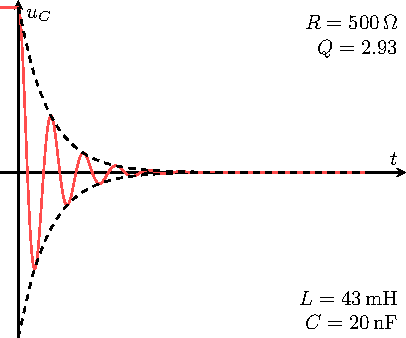
\includegraphics[width=\linewidth]{carac-rlc-3} &
	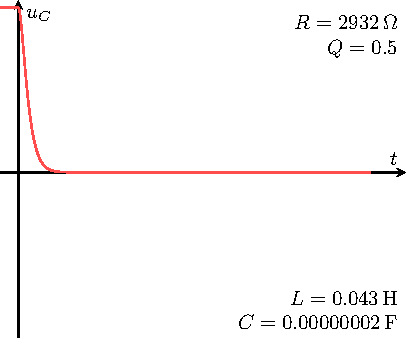
\includegraphics[width=\linewidth]{carac-rlc-05} &
	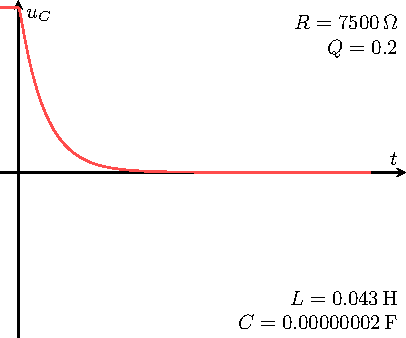
\includegraphics[width=\linewidth]{carac-rlc-02}
	\\\hline
	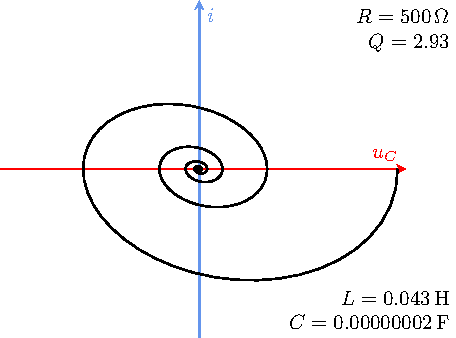
\includegraphics[width=\linewidth]{carac-rlc_xy-3} &
	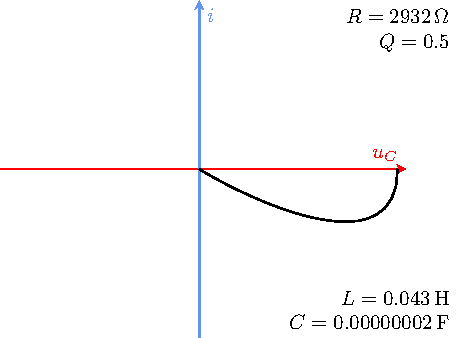
\includegraphics[width=\linewidth]{carac-rlc_xy-05} &
	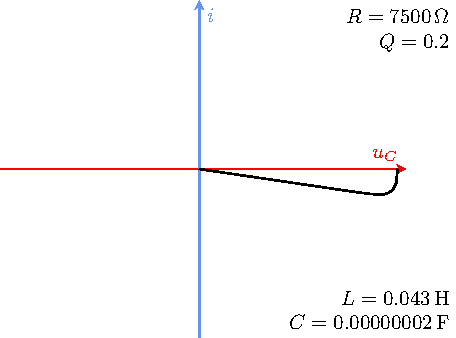
\includegraphics[width=\linewidth]{carac-rlc_xy-02}
	\\\hline
\end{tcb}

\end{document}
